%!LW recipe=LuaLaTeX (latexmk)

\documentclass[final]{beamer}

% ============================================================
% Packages
% ============================================================

\usepackage[size=custom,width=120,height=90,scale=1.0]{beamerposter}

\usepackage{lmodern}
\usepackage{lipsum}
\usepackage{raleway}

% Gemini theme
\usetheme{gemini}
\usecolortheme{gemini}

% Figures and graphics
\usepackage{graphicx}

% Tables
\usepackage{booktabs}
\usepackage{multirow}
\usepackage{colortbl}
\usepackage{arydshln}

% Mathematics
\usepackage{mathtools}
\usepackage{amsmath,amssymb,amsfonts,amsthm}

% TikZ and plots
\usepackage{tikz}
\usetikzlibrary{overlay-beamer-styles}
\usetikzlibrary{shapes}
\usetikzlibrary{positioning}

\usepackage{pgfplots}
\pgfplotsset{compat=newest}
\pgfplotsset{plot coordinates/math parser=false}

% Subfigures
\usepackage{subcaption}

% QR codes
\usepackage{qrcode}

% Bibliography
\usepackage[
    backend=biber,
    style=numeric,
    sorting=none,
    maxnames=99
]{biblatex}

% Add your bibliography file here
% \addbibresource{bibliography.bib}


% ============================================================
% Colors
% ============================================================

\definecolor{ucsdblue}{RGB}{1,49,82}


% ============================================================
% Custom commands
% ============================================================

% Bold zero
\newcommand{\bzero}{\ensuremath{\mathbf{0}}}

% Vector notation
\newcommand{\vect}[1]{\mathbf{#1}}

% Common operators
\newcommand{\real}{\mathbb{R}}
\newcommand{\N}{\mathbb{N}}
\newcommand{\unif}{\mathbb{U}}

% Example tilted notation
\newcommand{\tA}{\ensuremath{\tilde{A}}}
\newcommand{\tB}{\ensuremath{\tilde{B}}}
\newcommand{\tC}{\ensuremath{\tilde{C}}}

% Example bold letters
\newcommand{\bA}{\ensuremath{\mathbf{A}}}
\newcommand{\bB}{\ensuremath{\mathbf{B}}}
\newcommand{\bC}{\ensuremath{\mathbf{C}}}
\newcommand{\bZ}{\ensuremath{\mathbf{Z}}}

% Example calligraphic letters
\newcommand{\cA}{\ensuremath{\mathcal{A}}}
\newcommand{\cB}{\ensuremath{\mathcal{B}}}
\newcommand{\cC}{\ensuremath{\mathcal{C}}}

% Kronecker-product power notation
\newcommand*\circled[1]{%
    \tikz[baseline=(char.base)]{
        \node(
            char
        )[shape=rounded rectangle,draw,inner sep=0.6pt,minimum height=1.5ex]{#1};
    }%
}

\newcommand{\kronF}[2]{%
    {#1}^{\circled{\small{\ensuremath{#2}}}}
}

% ============================================================
% Poster dimensions
% ============================================================

% If you have N columns, choose \sepwidth and \colwidth such that
%
%   (N+1)*\sepwidth + N*\colwidth = \paperwidth
%
% The original poster uses three columns.

\newlength{\sepwidth}
\newlength{\colwidth}

\setlength{\sepwidth}{0.025\paperwidth}
\setlength{\colwidth}{0.30\paperwidth}

\newcommand{\separatorcolumn}{%
    \begin{column}{\sepwidth}
    \end{column}
}


% ============================================================
% Title
% ============================================================
\title{Modeling a 1D Discrete Element System with High Performance Computing}
\author[Your Name]{
    Shelby Pullen \inst{1}
    \and
    Dr. Boris Kramer \inst{1}
}

\institute[Your Institution]{
    \inst{1}
    Department of Mechanical and Aerospace Engineering,
    University of California San Diego
}

% ============================================================
% Document
% ============================================================
\begin{document}
\Large
% ============================================================
% Logos
% ============================================================
\addtobeamertemplate{headline}{}
{
    \begin{tikzpicture}[
        remember picture,
        overlay
    ]

        % Left logo
        \node[
            anchor=north west,
            xshift=2cm,
            yshift=-1.5cm
        ] at (current page.north west)
        {
            
\includegraphics[
                height=4cm
            ]{figures/UCSDLogo_JSOE_White.png}
        };

        % Right logo
        \node[
            anchor=north east,
            xshift=-2cm,
            yshift=-1.5cm
        ] at (current page.north east)
        {
            
\includegraphics[
                height=6cm
            ]{figures/UCSD_logo.png}
        };

    \end{tikzpicture}
}
% ============================================================
% Poster frame
% ============================================================
\begin{frame}[t]
\begin{columns}[t]
% ============================================================
% column1
% ============================================================

\separatorcolumn

\begin{column}{0.96\colwidth}


% ------------------------------------------------------------
% Background and Motivation
% ------------------------------------------------------------

\begin{block}{Background and Motivation}

\begin{itemize}
    \item How can nonlinear wave dynamics be exploited for impact mitigation?
    \item Polynomial springs in 1D mass spring damper chains can dissipate Kinetic Energy \cite{macnider_customizable_2025}.

    \begin{center}
    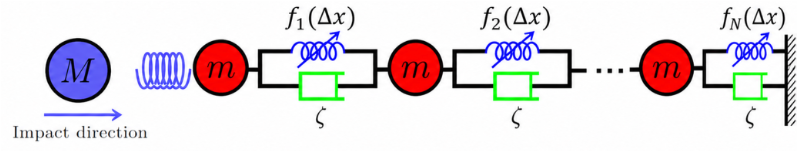
\includegraphics[
        width=0.9\linewidth
    ]{figures/1D_DEM_diagram.png}

    \vspace{0.4cm}

    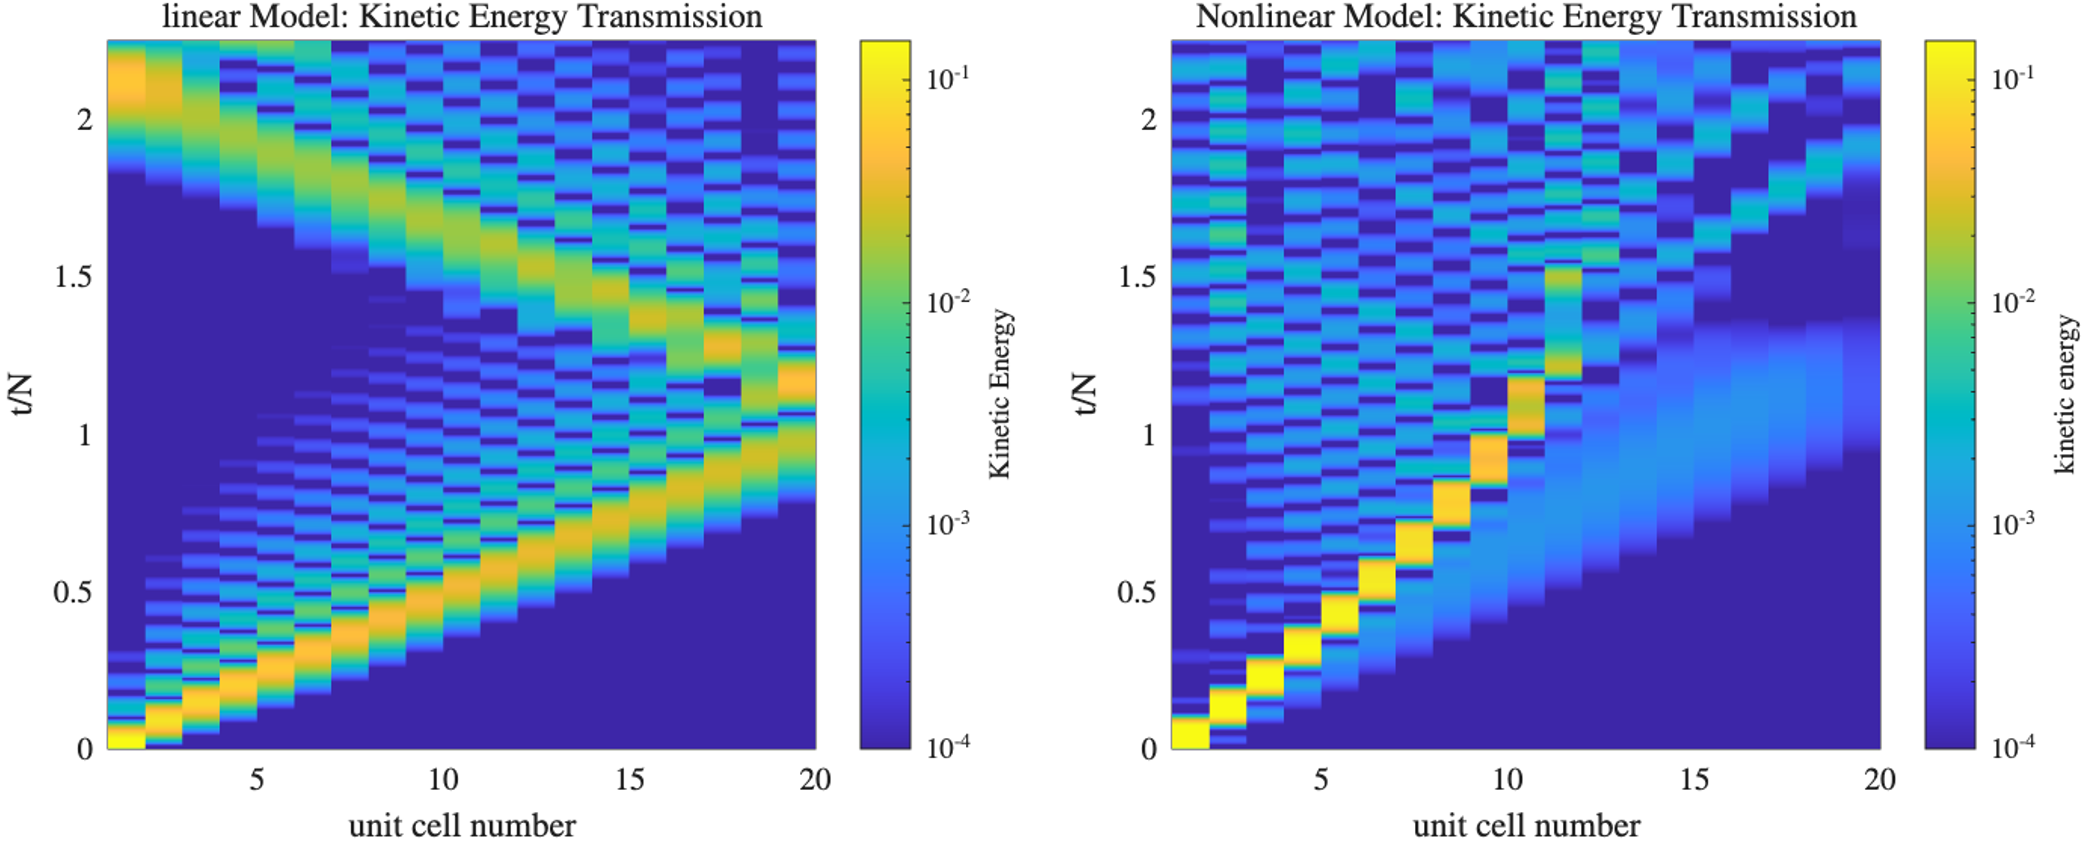
\includegraphics[
        width=0.9\linewidth
    ]{figures/background_KE_transmission.png}

    \end{center}

    \item Is there a robust nonlinear spring that can work for a range of impact conditions?

\end{itemize}
\vspace{0.5cm}
\end{block}

% ------------------------------------------------------------
% Research Problem
% ------------------------------------------------------------
\begin{alertblock}{Main Contributions}
\begin{center}
\textbf{
\begin{itemize}
    \item Forumated robust design optimization framework for the DEM
    \item Accelerated DEM compute time by porting to Python
    \item Exploited MC high throughput structure for parallelization
    \item Enabled multinode computing using built in SLURM job arrays
\end{itemize}
}
\end{center}
\end{alertblock}

% ------------------------------------------------------------
% Methods
% ------------------------------------------------------------
\begin{block}{Robust Design Optimization Problem}

\begin{equation}\label{spring}
\begin{aligned}
f_{\mathrm{non}}(x)
    &= c_1x
    + \textcolor{red}{c_2}x^2+\textcolor{red}{c_3}x^3,
\\[-0.1em]
f_{\mathrm{lin}}(x)
    &= c_1x.
\end{aligned}
\end{equation}

\vspace{-1.5cm}

\begin{equation}\label{KE_calc}
KE= \max_{t\geq 0}
       \left(\frac{1}{2}m\dot{x}_N^2\right),
\end{equation}

\vspace{-1.5cm}

\begin{equation}\label{KE_ratio_cal}
KE_{\mathrm{ratio}}
    \left(\textcolor{red}{c_2,c_3}; \textcolor{blue}{\bZ}\right)
    =
    \frac{
        KE_{\mathrm{non}}
        \left(
            \textcolor{red}{c_2,c_3};
            \textcolor{blue}{\bZ}
        \right)
    }{
        KE_{\mathrm{lin}}
        \left(
            \textcolor{blue}{\bZ}
        \right)
    }
\end{equation}

\vspace{-1.5cm}

\begin{equation}\label{Det_cost}
    (c_{2}^*, c_{3}^*) 
    = \arg\min_{(c_2,c_3)\in \mathcal{D}}KE_{ratio}(
    \textcolor{red}{c_2,c_3};\ 
    \textcolor{blue}{\bZ} )
\end{equation}

\vspace{-1.5cm}

\begin{equation}\label{RV_distribution}
    \textcolor{blue}{\bZ} = \begin{bmatrix} 
        \textcolor{blue}{\zeta} \\ 
        \textcolor{blue}{\frac{M}{M_0}} \\ 
        \textcolor{blue}{\frac{V}{V_0}}
    \end{bmatrix} \sim \unif \begin{pmatrix}
        [0.005, 0.025] \\ [0.030,0.080] \\ [0.500 ,1.100]
    \end{pmatrix}
\end{equation}

\vspace{-1.5cm}

\begin{equation}
    J\left(\textcolor{red}{c_2,c_3}\right)= 
    \mathbb{E} \left(KE_{ratio}\left( \textcolor{red}{c_2,c_3}; 
    \textcolor{blue}{\mathbf{Z}}\right)\right) 
    + \mathbb{V} 
    \left(KE_{ratio}\left(\textcolor{red}{c_2,c_3}; \textcolor{blue}{\mathbf{Z}}\right)\right)
\end{equation}

\vspace{0.5cm}

\end{block}

\end{column}

% ============================================================
% COLUMN 2
% ============================================================

\separatorcolumn

\begin{column}{1.01\colwidth}

% ------------------------------------------------------------
% Algorithm / Workflow
% ------------------------------------------------------------

\begin{block}{Algorithm or Workflow}
\vspace{0.cm}

\begin{center}

\begin{tikzpicture}[
    node distance=2cm,
    box/.style={
        draw,
        rounded corners,
        minimum width=5cm,
        minimum height=1.5cm,
        align=center
    },
    arrow/.style={
        ->,
        >=stealth,
        line width=4pt
    }
]

    \node[draw,rounded corners,minimum width=5cm,minimum height=1.5cm] (A)
    {
        Sample $\textcolor{blue}{\bZ}$
    };

    \node[draw,rounded corners,minimum width=5cm,minimum height=1.5cm] (B)
    [right=2cm of A]
    {
        obj func
    };

    \node[draw,rounded corners,minimum width=5cm,minimum height=1.5cm] (C)
    [right=2cm of B]
    {
        compute $KE_{\mathrm{ratio}}$
    };

    \node[draw,rounded corners,minimum width=5cm,minimum height=1.5cm] (D)
    [right=2cm of C]
    {
        $J\left(\textcolor{red}{c_2,c_3}\right)$
    };


    \draw[->,>=stealth,line width=4pt]
    (A) -- (B);

    \draw[->,>=stealth,line width=4pt]
    (B) -- (C);

    \draw[
        arrow,
        rounded corners
    ]
    (C.south)
        -- ++(0,-2cm)
        -| node[pos=0.25,below]
        {\normalsize for 1000 samples}
    (A.south);

    \draw[->,>=stealth,line width=4pt]
    (C) -- (D);

    \draw[
        arrow,
        rounded corners
    ]
    (D.south)
        -- ++(0,-4cm)
        -| node[pos=0.25,below]
        {\normalsize
        $\forall(\textcolor{red}{c_2,c_3})\in\mathcal{D}$
        }
    (A.south);

\end{tikzpicture}

\end{center}

\end{block}

% ------------------------------------------------------------
% Code Verification
% ------------------------------------------------------------

\begin{block}{Code Verification}

\vspace{0.5cm}

\begin{center}
    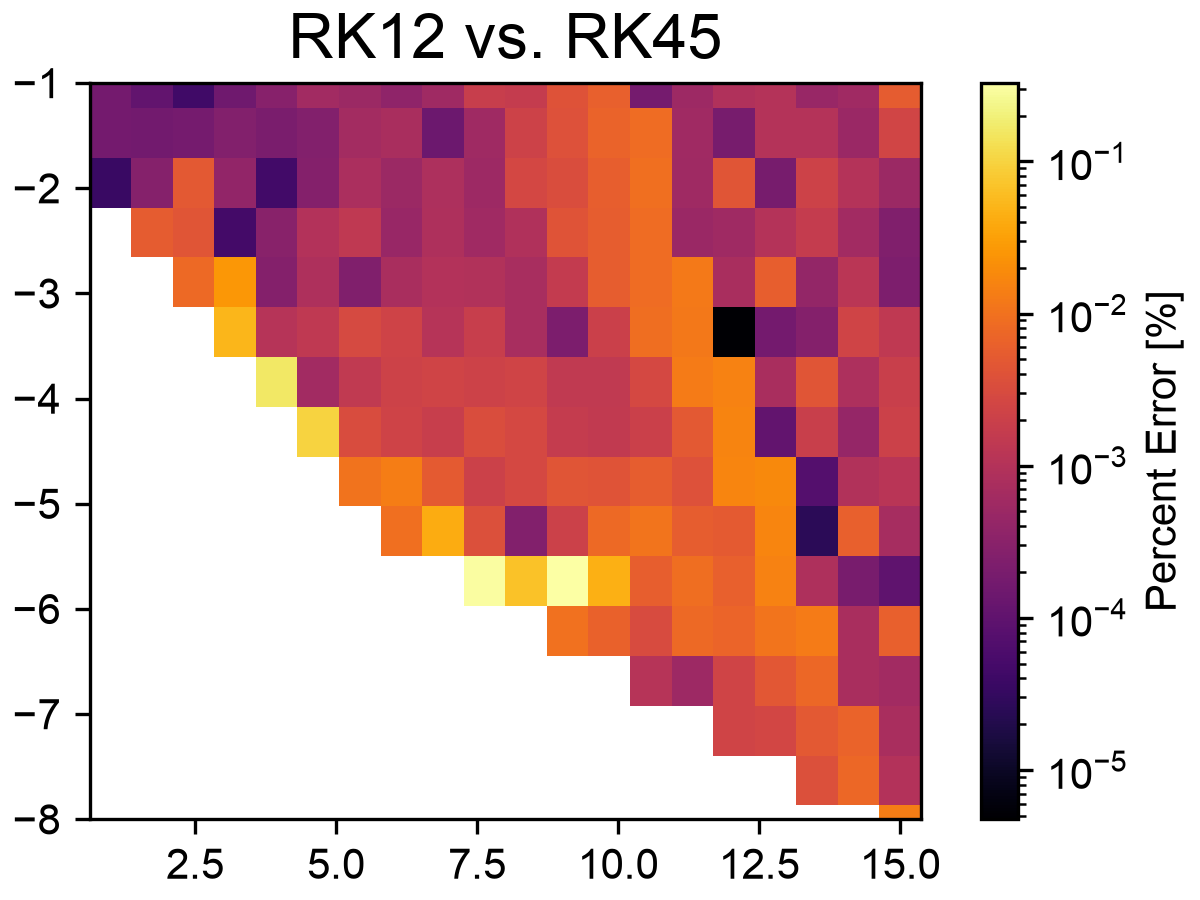
\includegraphics[
        width=0.5\linewidth
    ]{figures/RK12solver_conv_study.png}
\end{center}

\vspace{0.5cm}

\begin{center}
    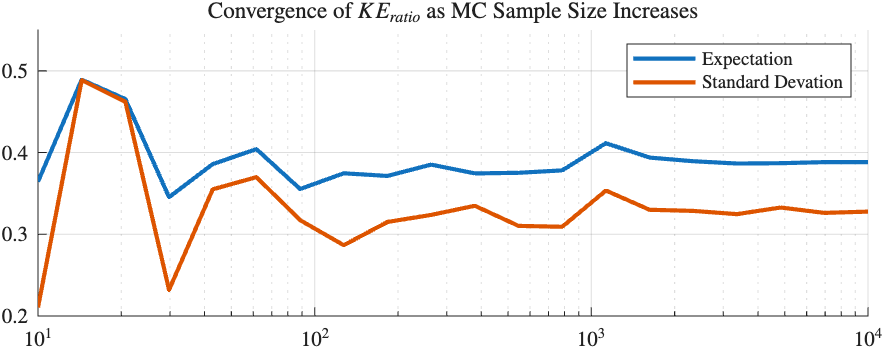
\includegraphics[
        width=0.9\linewidth
    ]{figures/LoLN_both.png}
\end{center}

\begin{center}
   
% table of det 20x20 speed up
\begin{table}

\centering

\begin{tabular}{|l|c|c|c|}

\hline

\rowcolor[rgb]{0.941,0.941,0.941}

\textbf{20x20}  &   \textbf{Matlab}    &   \textbf{Python Local}  &   \textbf{Python Dane}
\\

\hline

$KE_{\mathrm{ratio}}$ &   1.00         &   0.80                   &   20
\\

\hline

opt Coeffs            &   2.10         &   1.40                   &   33
\\

\hline

CPU hrs               &   4.50         &   3.20                   &   29
\\

\hline

Wall Clock Time       &   8.20         &   5.10                   &    38
\\

\hline

\end{tabular}

\end{table}

\end{center}

\end{block}

\end{column}

% ============================================================
% COLUMN 3
% ============================================================

\separatorcolumn

\begin{column}{1.05\colwidth}


% ------------------------------------------------------------
% Results Table
% ------------------------------------------------------------

\begin{block}{Deterministic Results}

\vspace{0.cm}

\begin{center}
    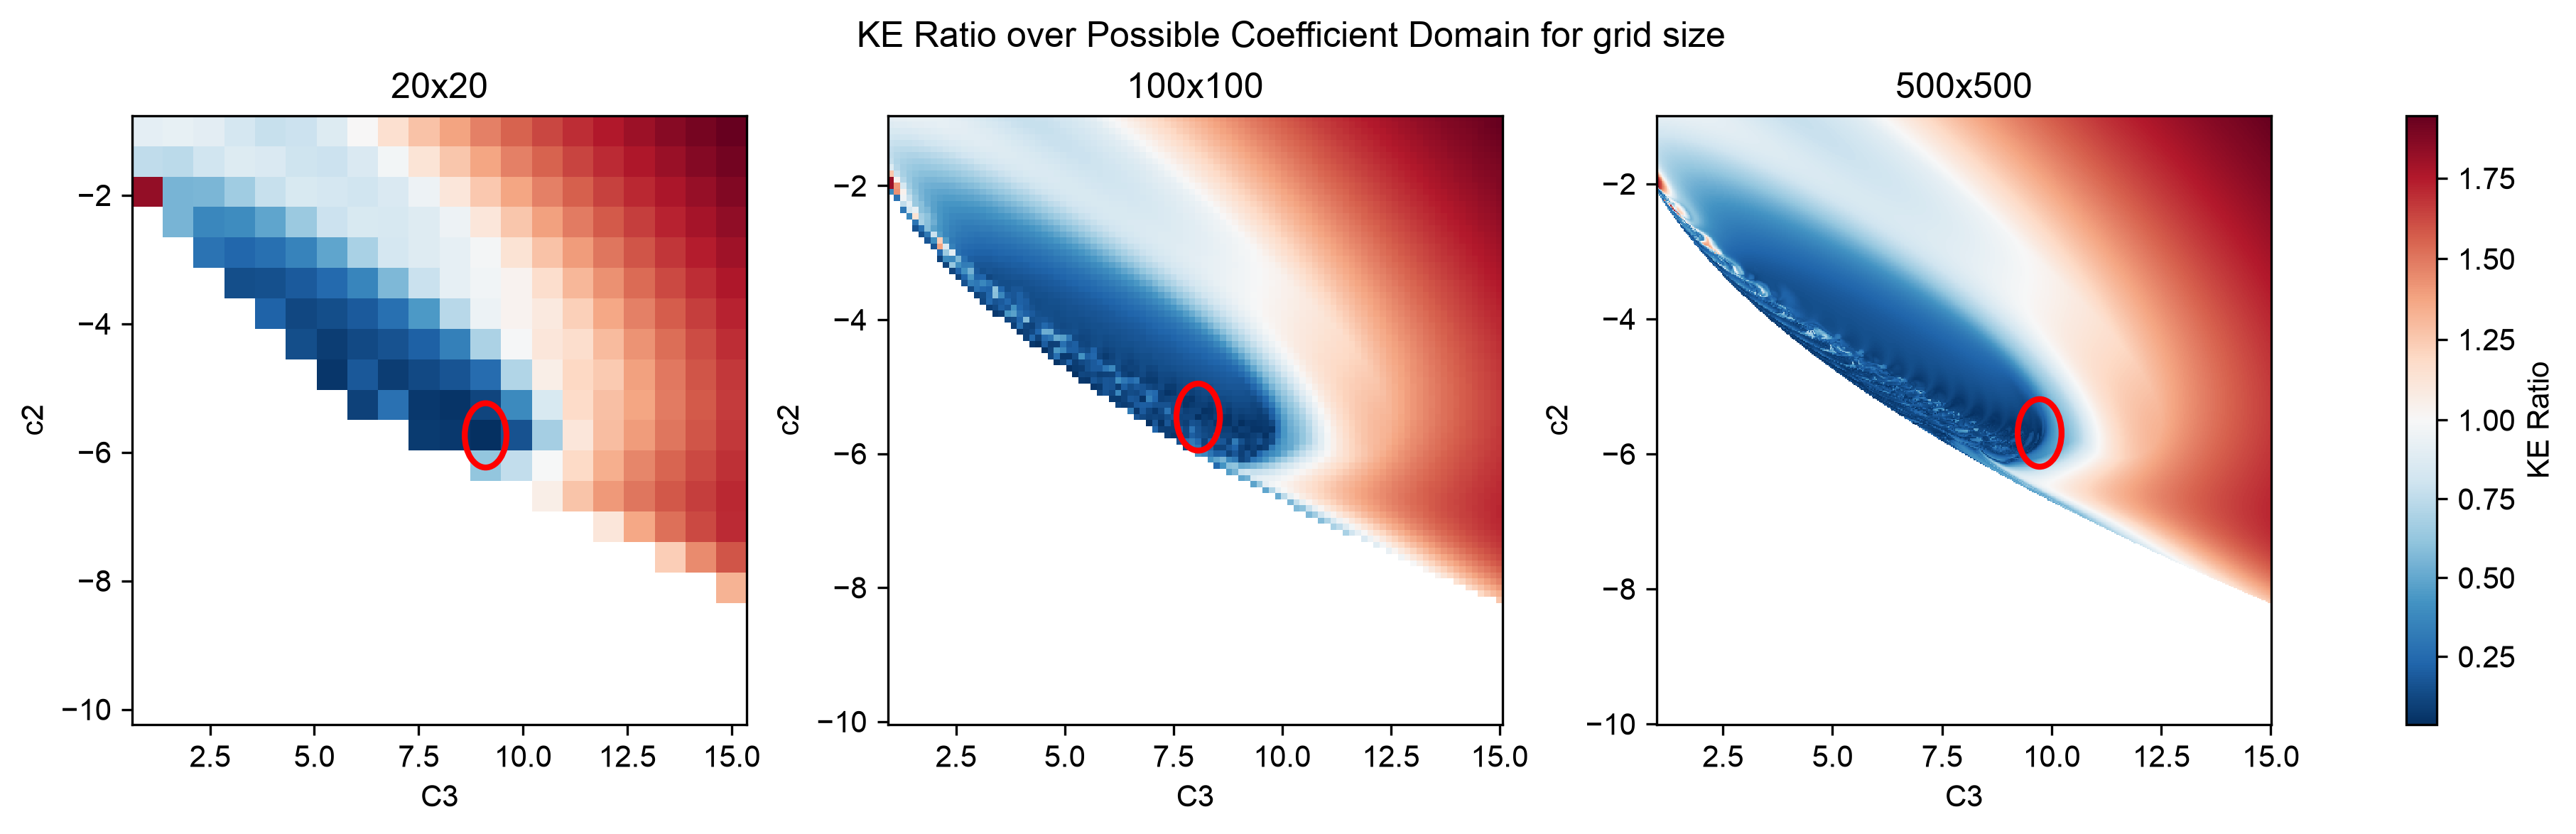
\includegraphics[
        width=0.9\linewidth
    ]{figures/det_grid_ref_comp.png}
\end{center}

\vspace{0.5cm}

\begin{center}
    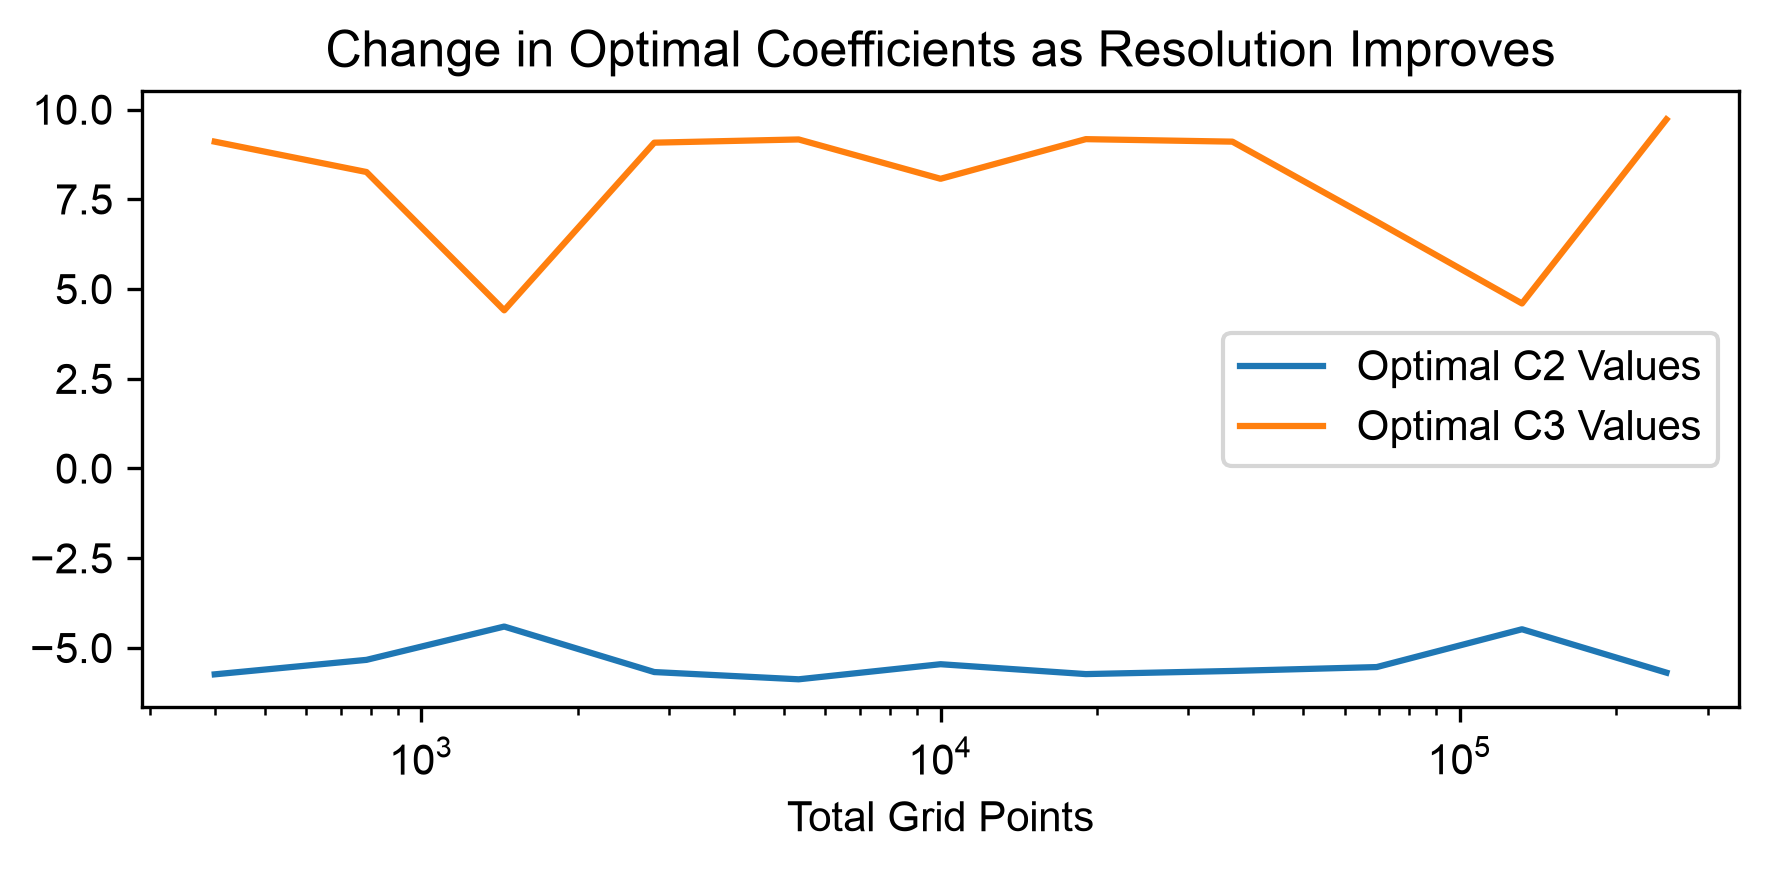
\includegraphics[
        width=0.4\linewidth
    ]{figures/optimal_coeff_values_grid_ref.png}
\end{center}

% \begin{center}
%     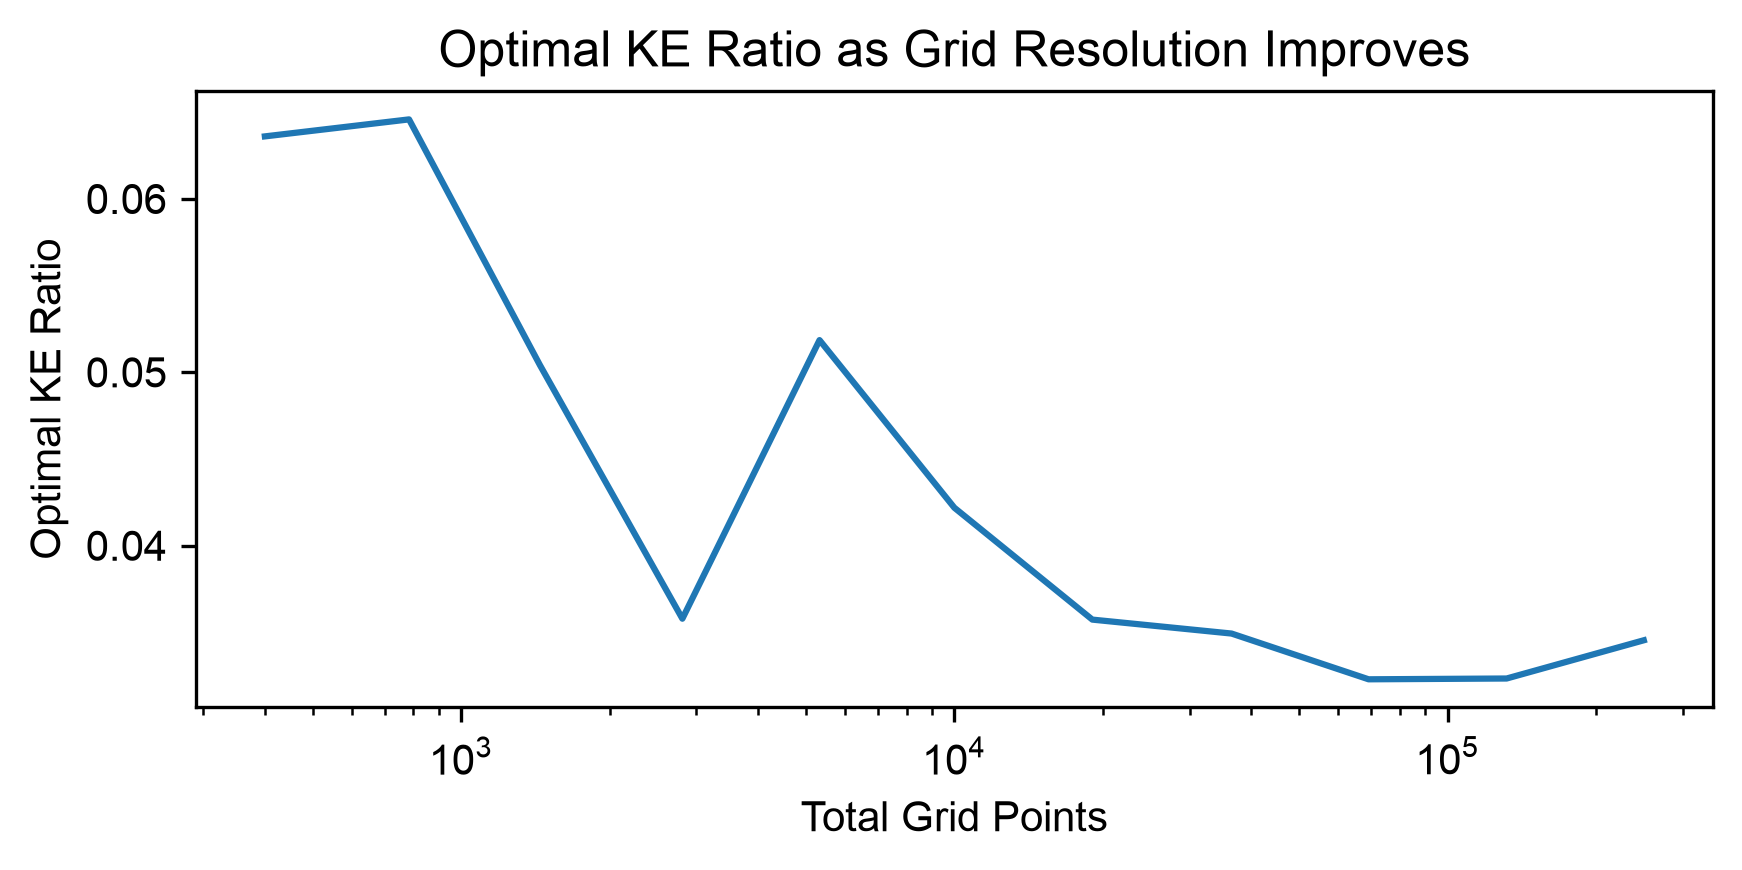
\includegraphics[
%         width=0.4\linewidth
%     ]{figures/optimal_KE_values_grid_ref.png}
% \end{center}

\end{block}
\vspace{-0.5cm}
% ------------------------------------------------------------
% Results Figure
% ------------------------------------------------------------

\begin{block}{Monte Carlo Estimate Results}

\begin{center}
    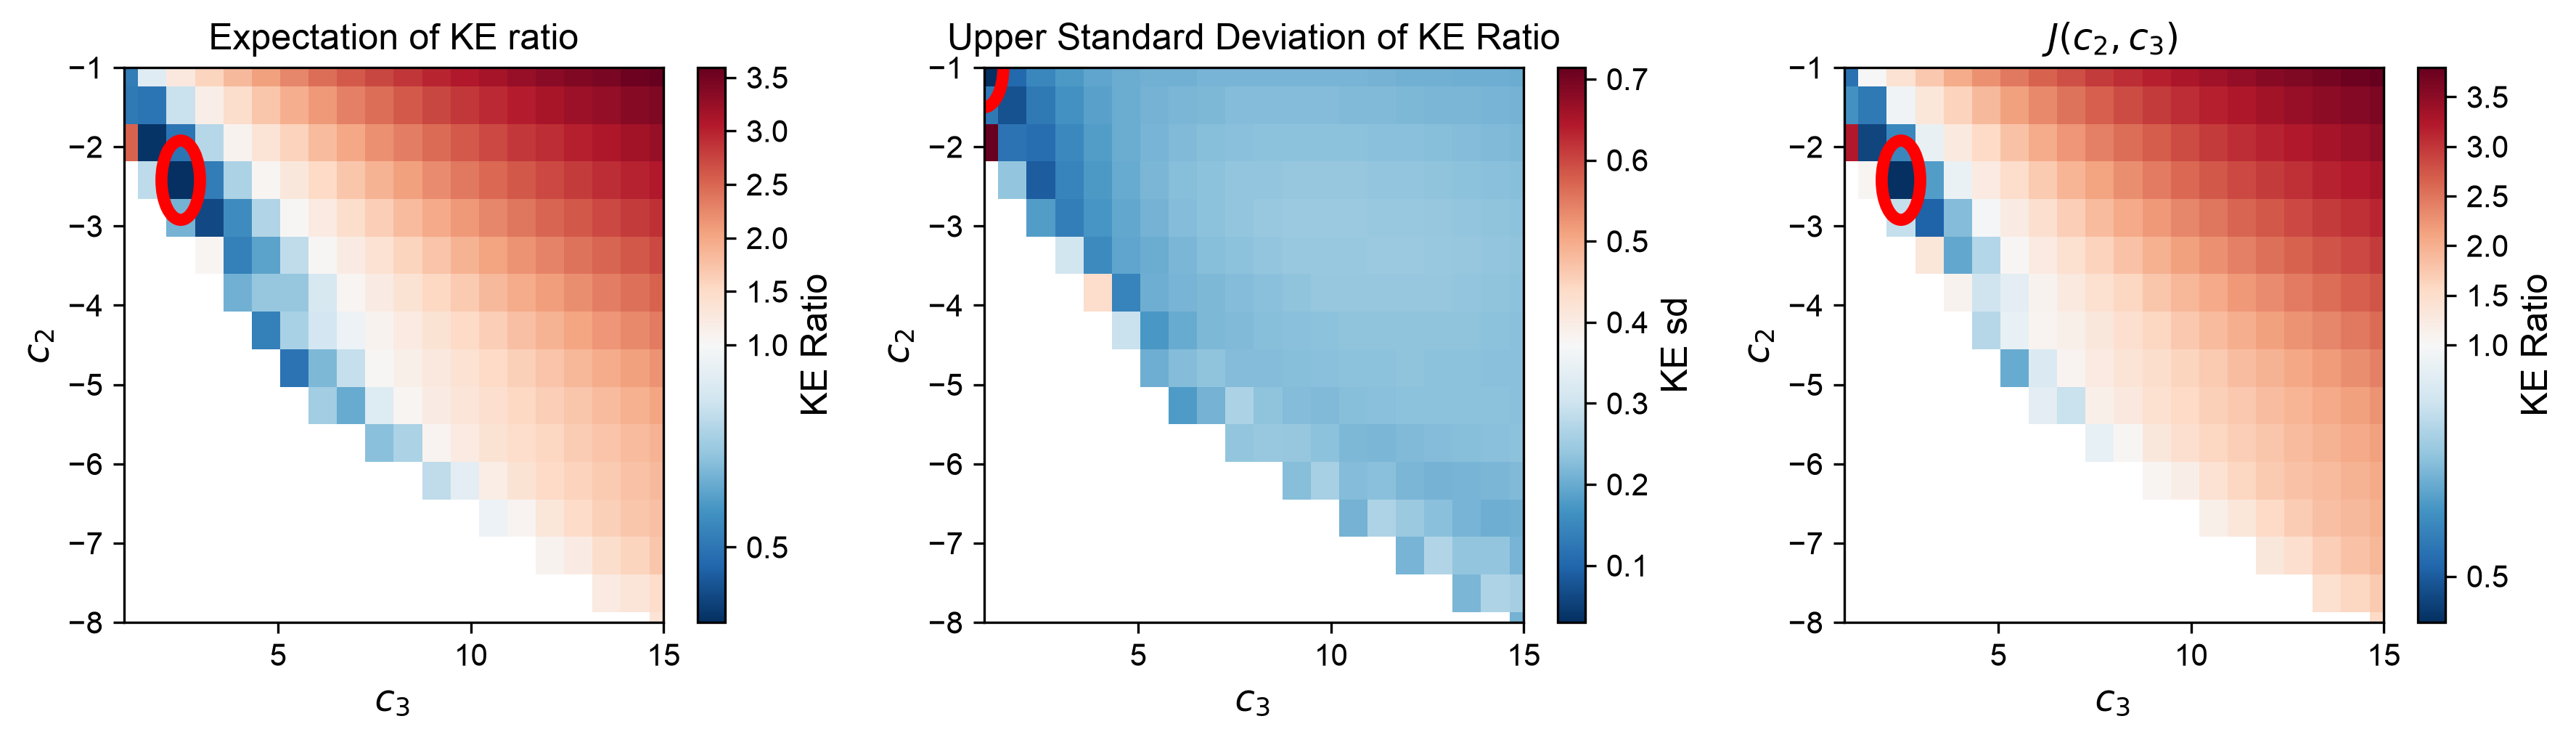
\includegraphics[
        width=0.9\linewidth
    ]{figures/most_refined_20x20_KE_avgs.png}
\end{center}

\begin{center}
   
% table of rob 20x20 speed up
\begin{table}

\centering

\begin{tabular}{|l|c|c|c|}

\hline

\rowcolor[rgb]{0.941,0.941,0.941}

\textbf{20x20}  &   \textbf{Matlab}    &   \textbf{Python Local}  &   \textbf{Python Dane}
\\

\hline

$KE_{\mathrm{ratio}}$ &   1.00         &   0.80                   &   20
\\

\hline

opt Coeffs            &   2.10         &   1.40                   &   33
\\

\hline

CPU hrs               &   4.50         &   3.20                   &   29
\\

\hline

Wall Clock Time       &   8.20         &   5.10                   &    38
\\

\hline

\end{tabular}

\end{table}

\end{center}

\textbf{include refined MC sampled figure with cpuhr below}

\end{block}

% ------------------------------------------------------------
% Summary
% ------------------------------------------------------------

\begin{block}{Summary and Future Work}

\begin{itemize}
    \item 2D DEM
    \item Experimental Validation of Impact Distributions
\end{itemize}

\end{block}
\vspace{-1.cm}

% ------------------------------------------------------------
% QR Code
% ------------------------------------------------------------

\begin{center}

\Large
\textbf{Project / Software}

\vspace{0.3cm}

% Replace the URL with your own.
\qrcode[
    height=2in
]{https://github.com/shelbypullen/SHAPE-UQDEM-Py}

\vspace{0.3cm}

\large
Scan for more information

\end{center}


% ------------------------------------------------------------
% Acknowledgements
% ------------------------------------------------------------

\begin{block}{Acknowledgements}

This work was supported by

\textbf{
    [funding agency / grant number / collaborators].
}

\end{block}
\vspace{-1cm}

% ------------------------------------------------------------
% References
% ------------------------------------------------------------

\begin{block}{References}

% Uncomment the following line once you have a bibliography:
%
\printbibliography

\end{block}


\end{column}


% ============================================================
% Final separator
% ============================================================

\separatorcolumn

\end{columns}

\end{frame}

\end{document}